%& --translate-file=il2-cs
\documentclass[a4paper,12pt,oneside,notitlepage,openright]{report} %print on both side

%%%%%%%%%%%%%%%%%%%
%%%% PREAMBULE %%%%
%%%%%%%%%%%%%%%%%%%
\usepackage[utf8]{inputenc} 		% neco kvuli cestiny :) \
\usepackage[IL2]{fontenc}			% neco kvuli cestiny :)  | - nevim, co na to windows :)
\usepackage[czech]{babel}   		% neco kvuli cestiny :) /
\usepackage{a4wide} 				% aby byl text sirsi ... vpodstate tedy normalni
\usepackage{indentfirst}			% pro odsazeni prviho odstavce

%%%%%% Printing code
%\usepackage[scaled]{beramono}
%\renewcommand*\familydefault{\ttdefault}
\usepackage{listings}
\renewcommand\lstlistingname{Ukázka kódu}
\renewcommand\lstlistlistingname{Ukázky kódu}
%The first changes the caption name for listings. The second — the header name for the list of listings which is printed by the \lstlistoflistings command.
\def\lstlistingautorefname{Ukázka kódu}

\lstset{
  language=Python,
  basicstyle=\footnotesize,
  numberstyle=\tiny\color{gray},
  frame=single,
  keywordstyle=\color{black}\textbf,
  showstringspaces=false,
  captionpos=b,
  formfeed=\newpage,
  tabsize=3,
  commentstyle=\itshape,
  stringstyle=\ttfamily,
  numbers=left
  %morekeywords={models, lambda, forms}
}


%%%%%% Literature
\usepackage{biblatex}
\bibliography{thesis}

%%%%%% tady jsem nastavoval okraje pro tisknuti, snad to tak muze byt :)
\setlength{\oddsidemargin}{0mm} 
\setlength{\textwidth}{155mm}\setlength{\topmargin}{0mm} 
\setlength{\textheight}{230mm}
\setlength{\headheight}{14.5pt}         %height of head
\setlength{\oddsidemargin}{7mm}         %odd left margin
\setlength{\evensidemargin}{-\oddsidemargin} %even left margin

% balicek pro tvorbu indexu - myslim, ze je zde standardne
\usepackage{index}	% pro tvorbu rejstriku
\newindex{default}{idx}{ind}{Rejstřík}

% to je neco pro tvorbu odkazu a nacitani obrazku
\usepackage[pdftex]{hyperref}
\usepackage[pdftex]{graphicx}
\renewcommand{\figurename}{Obr.}
\addto\captionsczech{\renewcommand{\figurename}{Obr.}}

% barevny text
\usepackage{color}
\definecolor{gray}{rgb}{0.5,0.5,0.5}

\def \u{1.5}

%%%% zahlavi, zapati .... da se s tim pekne pohrat
\usepackage{fancyhdr}
\fancyhf{}
\fancyfoot[C]{\thepage} 
\fancyhead[L]{\slshape \leftmark}
\renewcommand{\headrulewidth}{0.4pt} 
\renewcommand{\footrulewidth}{0.0pt}    

%%%% tabulka - vice radku v bunce
\usepackage{multirow}

% nastaveni radkovani na 1.5 radku
\def\baselinestretch{1.5}\normalsize
\begin{document}
%-----<<< TITULNI STRANA >>>-----
%-----<<< TITLE PAGE >>>-----
\def \CVUT {České vysoké učení technické v~Praze}
\def \FSV {Fakulta stavební}
\def \KATEDRA {Katedra mapování a kartografie}
\def \BookName {DIPLOMOVÁ PRÁCE}
\def \Bookname {Workflow Builder}
\def \Authors {Zdeněk Růžička}
\def \DatumDP {Praha, 2012}
\newcommand{\vedouci}{Ing. Martin Landa, Ph.D.}
% TODO: ask Martin, if he is Ph.D. or not yet

\def \BookHeadDP {
    \begin{center}
    {\LARGE \textsc \CVUT}\\[2ex]
    {\LARGE \textsc \FSV}\\

    \vspace{2cm}
	\begin{center}
		
\includegraphics[scale=0.55]{pictures/lev}
	\end{center}
    \vspace{1cm}

    {\textbf {\Huge \BookName \\[4ex]}
    {\LARGE \bf \Bookname}
    }

   \vfill
   {\large
    \begin{tabular}{rl}
    Vypracoval: & \Authors\\
    Vedoucí práce: & \vedouci\\
    Rok: & \DatumDP
    \end{tabular}
   }

    \newpage
    \end{center}
}
\pagestyle{empty}                       %no pagination
\BookHeadDP
\cleardoublepage

%-----<<< ---------- >>>-----
%%-----<<< ---------- >>>-----
%
%%-----<<< PROHLASENI >>>-----
\pagestyle{plain}                       %no pagination
\pagenumbering{roman}                   %start roman pagination from 1
\setcounter{page}{2}
\vfill

\vglue 13cm

\section*{Prohlášení}
\indent\indent Prohlašuji, že jsem svou diplomovou práci na téma \textbf{Workflow Builder} vypracoval samostatně s pomocí svého vedoucího práce a za použití literatury a zdrojů uvedených v~přiloženém seznamu na konci práce.
\vspace{0.5cm}

%\iffalse
%\noindent Nemám závažný důvod proti užití  tohoto
%školního díla ve smyslu § 60 Zákona č.121/2000 Sb. , o~právu
%autorském, o~právech souvisejících s~právem autorským a o~změně
%některých zákonů (autorský zákon). {\em Tento odstavec je
%nepovinný, záleží na vašem rozhodnutí.}
%\fi

\begin{table}[!hbp]
\begin{tabular}{lr}
  V~Praze dne
  \begin{tabular}{p{2.5cm}}
    \\
    \hline
  \end{tabular}
 &
 \hspace{4cm}
 \begin{tabular}{p{3.5cm}}
    \vspace{0.6cm} \\
     \hline \hspace{1cm} podpis
 \end{tabular}

\end{tabular}
\end{table}

\newpage
%%-----<<< ---------- >>>-----
%
%%-----<<< PODEKOVANI >>>-----
\vfill

\vglue 14cm

\section*{Poděkování}
\indent\indent Především děkuji vedoucímu mé diplomové práce Ing. Martinu Landovi za
odborné vedení, rychlé reakce na mé dotazy a ochotu hledat na ně
odpovědi. Dále bych chtěl poděkovat Camilo Polimeris za napsání QGIS
Processing Frameworku, jehož je tato práce součástí. V neposlední řadě
bych chtěl poděkovat rodině a kamarádům za důvěru a podporu během
studií.
          %input file
\cleardoublepage
%%-----<<< ---------- >>>-----
%
%%-----<<< ABSTRAKT >>>-----
\section*{Abstrakt}\label{abstrakt}
\indent Diplomová práce si vytyčila za cíl vytvořit v prostředí
Quantum GIS (dále jen QGIS) nástroj, který by umožňoval uživateli
grafické propojování modulů z frameworku \textbf{QGIS Processing
  Framework}. V úvodní kapitole je představena knihovna Qt, resp. její
verze PyQt pro jazyk Python, ve které byl celý \textbf{Workflow
  Builder} napsán. Dále je představeno prostředí QGIS a popsána práce
s QGIS Processing Frameworkem.

V druhé kapitole diplomové práce je představena samotná aplikace
Workflow Build\-er.

V poslední kapitole je zmínka o frameworku \textbf{SEXTANTE}, který se
objevil v konci psaní této práce.

\textbf{Klíčová slova}

Quantum GIS, QGIS, workflow, open source, GIS, PyQt, QGIS Processing Framework


\vfill

\section*{Abstract}
\indent The goal of this master thesis is to create a tool for Quantum GIS 
that would give user possibility to chain modules from \textbf{QGIS Processing 
Framework}. In the first chapter graphical library Qt and its binding for Python 
(PyQt) is introduced. \textbf{Workflow Builder} was written in PyQt. Quantum GIS and 
QGIS Processing Framework are also introduced.

In the second chapter of the thesis is descibed a work with the 
Workflow Builder. In the last chapter is mentioned framework \textbf{SEXTANTE} 
that appeared at the end of work on this thesis.

\textbf{Key words}

Quantum QGIS, workflow, open source, GIS, PyQt, SAGA, QGIS Processing Framework
          %input file
\cleardoublepage
%%-----<<< -------- >>>-----
%
%%-----<<< ZADÁNÍ DIPLOMOVÉ PRÁCE >>>-----
%ZADANI - original
\cleardoublepage
%%-----<<< ---------------------- >>>-----
%
%%-----<<< TABLE OF CONTENTS >>>-----
\setcounter{secnumdepth}{4}             %number of section to 4
\setcounter{tocdepth}{4}                %number of section in table of contents greater then 3
\tableofcontents
\cleardoublepage
%%-----<<< ----------------- >>>-----
%
%%-----<<< TABLE OF CONTENTS PAGINATION >>>-----
\pagenumbering{arabic}                  %start arabic pagination from 1
%%-----<<< ---------------------------- >>>-----
%
%
%%-----<<< CHAPTERS >>>-----
\hyphenation{Automatica}                %no divide words
\pagestyle{fancy}

\chapter*{Úvod}
\addcontentsline{toc}{chapter}{Úvod}

V dnešní době se můžeme setkat s \index{GIS} geoinformačními ( GIS ) technologiemi na každém kroku. V různých oblastech krajinného inženýrství, při plánování výstavby silnic, v územním plánování, při řešení krizových situacích či plánování záchranných akcí. Uživatel si může vybrat z nepřeberného množství již existujících GIS nástrojů, řešení. A s potěšením lze konstatovat, že svobodná řešení, nejen v oblasti geoinformačních technologií, drží krok s těmi proprietárními. Uživatel tedy nemusí sahat hluboko do kapsy. Co se týče nástrojů pro prohlížení, zpracování a analýzu \index{geodata} geodat, můžeme jmenovat například GRASS GIS, gvSIG, Quantum GIS či SAGA GIS. Tato práce si ale nekladla za cíl srovnat GIS nástroje, ale implementaci nástroje do programu Quantum GIS, který by uživateli umožňoval vytvářet vlastní funkce spojováním již existujících funkcí.

Můžeme se také setkat s pojmy jako \begin{scriptsize}model builder\end{scriptsize} či \begin{scriptsize}chaining\end{scriptsize}. V této práci bude používán pojem workflow builder. Tento název byl převzat z projektu \index{VisTrails} VisTrails, který byl inspirací pro grafiku. Takzvané workflow buildery dávají uživateli možnost vytvářet si vlastní moduly za pomocí spojování výstupů a vstupů modulů již existujících. Uživatel tak nemusí spouštět každý modul zvlášť a starat se o výstupy, nová data, která se vytvoří jen dočasně a která uživatel v konečném výsledku nepotřebuje. Dále je pro uživatele mnohem pohodlnější, pakliže může najít všechny funkce na jednom místě (tzv. toolbox), nežli při hledání procházet všechny možné pluginy.

V době psaní této diplomové práce existoval projekt \index{QGIS Processing Framework} QGIS Processing Framework studenta Camilo Polymeris z univerzity Universidad de Concepción. QGIS Processing Framework si kladl za cíl být frameworkem, který by sdružoval moduly z pluginů pro QGIS na jednom místě. Odtud by byly jednotlivé moduly volány, pomocí workflow builderu spojovány, ukládány atp. V rámci tohoto projektu začala vznikat podpora pro použití modulů z jiného GIS nástroje - \index{SAGA GIS}System for Automated Geoscientific Analysis ( SAGA GIS ). V době psaní této práce existovala podpora pro 170 modulů, ne všechny ale byly testovány a fungovaly správně. I přesto se mohlo začít s prací na workflow builderu.

Aktuální verzi workflow builderu můžete najít zde:

\begin{center}
	\href{https://github.com/CzendaZdenda/qgis}{\texttt{https://github.com/CzendaZdenda/qgis}}
\end{center}              %input files
\chapter{Teorie}
V první části této kapitoly představím programovací jazyk Python, ve kterém byl napsán Workflow Builder. Jazyk Python je v dnešní době stále více oblíbený a můžeme ho najít snad všude, kam se podíváme. V druhé čáasti této kapitole představím jeden ze svobodných systémů pro práci s geografickými daty - Quantum GIS a možnost rozšiřování funkcionality pomocí zásuvných modulů, tzv. pluginů. To bylo původně možné jen v jazyce C++. Již nějakou dobu je také možné psát pluginy v jazyce Python, což přineslo výhody v podobě jednoduché šiřitelnosti (není nutná kompilace) a snažšího vývoje pluginů. V další části se budu věnovat knihovně Qt, respektive její verze pro jazyk Python - PyQt4. Zde popíši nástroje, které jsem využil při psaní Workflow Builderu. Mezi tyto nástroje patří hlavně implementace architektury MVC v podobě model-view-delegate, Graphics View Framework pro vykreslování a správu grafických prvků, signály a sloty pro komunikaci mezi objekty knihovny Qt a mechanismus Drag and Drop. V předposlední části popíši projekt QGIS Processing Framework, co bylo jeho cílem, jeho koncem a také možnosti jeho rozšiřování.  V poslední části představím modul xml.dom jazyka Python pro práci s objekty ve formátu XML.

\newpage
\newpage
\section{Python}
\index{Python}
\nocite{py3:book}

Python je interpretovaný, procedurální a objektově orientovaný jazyk, ve kterém se rychle programuje. Existuje pythoní verze Qt - PyQt.
\section{Quantum GIS}

\nocite{qgis:www}
\index{QGIS,Quantum GIS}

\begin{center}
	
\includegraphics[scale=0.1]{pictures/qgis_logo}
\end{center}

Quantum GIS je nejen prohlížečka geografických dat dostupná pro MS Windows, GNU/Linux, Unix, BSD a Mac OS X. Quantum GIS podporuje díky knihovně \index{OGR}OGR většinu vektorových formátů dat jako například ESRI Shapefile, GRASS, MapInfo či GML a díky knihovně \index{GDAL} GDAL mnoho rastrových formátů jako TIFF, ArcInfo, GRASS raster, ERDAS a další. Přes Quantum GIS můžeme také přistupovat k datům uložených v geodatabázích PostGIS a SpatiaLite či k datům dostupných přes WMS a WFS služby. Quantum GIS je šířen pod licencí GNU Public Licence. \footnote{http://qgis.org/about-qgis/features.html}

Program je napsán v jazyce C++. Poslední stabilní verze nese označení 1.7.4. Quantum GIS je lehce rozšířitelný program pomocí pluginů, které mohou být psány na jazyce Python nebo C++. Quantum GIS má poměrně dobře zdokumentované API a nutno také podotknout, že komunita kolem Quantum GISu je aktivní a podpora skrze mailinglisty je na vysoké úrovni.

Systém začal vyvíjet v roce 2002 Gary Sherman. Mělo jít o nenáročnou prohlížečku geodat pro Linux s širokou podporou datových formátů. Dlouhou dobu byl Quantum GIS brán převážně jako grafická nadstavba pro jiný desktopový GIS - GRASS GIS. Přes GRASS Plugin QGIS zpřístupňuje řadu modulů GRASS GIS. V současnosti se na vývoji nejvíce podílí skupina vývojářu kolem organizace \footnotemark{\index{Faunalia} Faunalia}\footnotetext{http://www.faunalia.co.uk/quantumgis}.

Funkcionalitu Quantum GIS rozšiřuje množství pluginů. Jako základní pluginy bych označil \footnotemark{\index{fTools} \textbf{fTools}} \footnotetext{http://www.ftools.ca/}, který umožňuje pokročilé prostorové analýzy nad vektorvovými daty, \footnotemark{\index{GDAL, GdalTools} \textbf{GdalTools}} \footnotetext{http://www.faunalia.co.uk/gdaltools} pro práci s rastrovými daty a již zmíňený \footnotemark{\index{GRASS Plugin} \textbf{GRASS Plugin}} \footnotetext{http://grass.osgeo.org/wiki/GRASS\_and\_QGIS} plugin, který zpřístupňuje funkce GRASSu uživatelům Quantum GIS. 

\subsection{Správa pluginů}
Jak už bylo zmíněno Quantum GIS umožňuje uživatelům rozšiřovat funkce programu dle jejich potřeb v podobě zásuvných modulů. Díky dobře zdokumentovanému API může uživatel pohodlně psát pluginy v jazyce C++ nebo Python. Pluginy píší jak vývojáři Quantum GISu, tak i obyčejní uživatelé. Pluginy si můžete stáhnout z oficiálních či neoficiálních repositářů. Pro instalování pluginů napsaných v jazyce Python a správu repositářů slouží nástroj \textbf{QGIS Python Plugin Installer}, dostupný přes \textit{Plugins $\rightarrow$ Fetch Python Plugins...}.

\begin{figure}
	\centering
	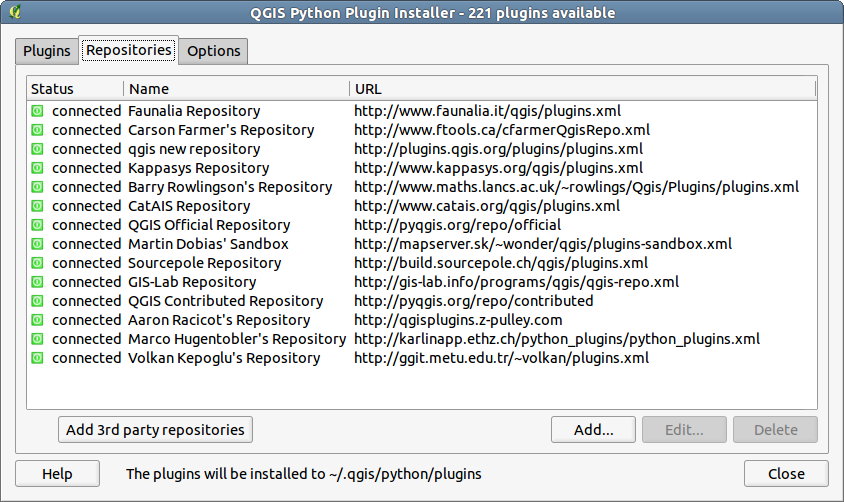
\includegraphics[scale=0.5]{pictures/qgis_plugin/python_installer}
	\caption{QGIS Python Plugin Installer - správa repozitářů}
  	\label{pythonplugininstaller}
\end{figure}


\noindent Jak je vidět z [Obr. \ref{pythonplugininstaller}], takto nainstalované pluginy se stáhnou do adresáře: 

\begin{itemize}
	\item \textit{\$HOME$\setminus$.qgis$\setminus$python$\setminus$plugins} - v případě OS GNU/Linux
	\item \textit{C:$\setminus$Documents and Settings$\setminus$USER$\setminus$.qgis$\setminus$python$\setminus$plugins} - v případě OS Windows bývá cesta podobná této
\end{itemize}

Pakliže uživatel napíše plugin v jazyce Python, doporučuji ho uložit do tohoto adresáře. Je také sice možnost uložit plugin do adresáře \textit{\$QGIS\_INSTALL\_DIR $\setminus$share$\setminus$qgis$\setminus$python$\setminus$plugins}, ale při případné opětovné kompilaci by byly změny ztraceny.

\noindent Pluginy psané v C++ se po přeložení ukládají standardně v \textit{\$QGIS\_INSTALL\_DIR $\setminus$lib$\setminus$qgis$\setminus$plugins} případně uživatel může přidat nová úložiště pomocí \textit{Settings $\rightarrow$ Options} a v záložce \textit{Generals} zadat cestu [Obr. \ref{cpprepository}].

\begin{figure}
	\centering
	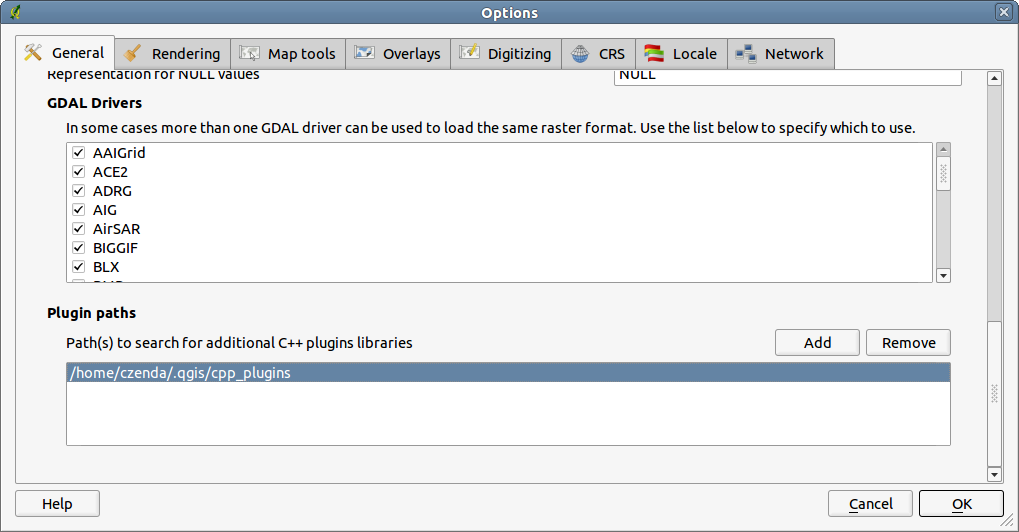
\includegraphics[scale=0.5]{pictures/qgis_plugin/options_cpp_path}
	\caption{\textit{Settings$\rightarrow$Options$\rightarrow$Generals} - přidání nové cesty k pluginům psaných na jazyce C++}
  	\label{cpprepository}
\end{figure}

Všechny nainstalované pluginy, ať psané v jazyce C++ či Python, může uživatel spravovat přes \textbf{QGIS Plugin Manager} - \textit{Plugins$\rightarrow$Manage Plugins...} [Obrázek \ref{plugin_manager}.

\begin{figure}
	\centering
	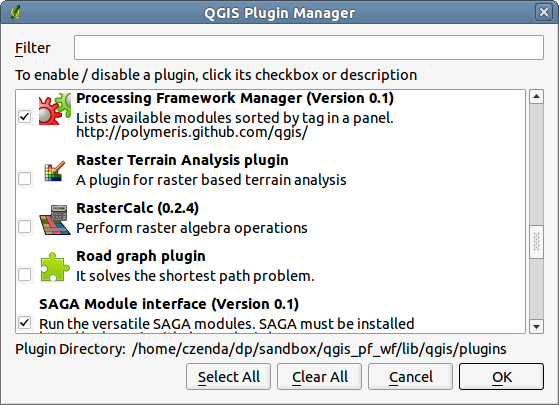
\includegraphics[scale=0.5]{pictures/qgis_plugin/plugin_manager}
	\caption{\textit{Plugins $\rightarrow$Manage Plugins...} - správa pluginů}
  	\label{plugin_manager}
\end{figure}

\subsection{Psaní vlastního pluginu}
Pluginy mohou být psány na jazyce C++ a Python. Již z charakteristiky daných jazyků vyplývá, že pro jednoduché, nenáročné či na začátku vývoje pluginy, se bude hodit spíše jazyk Python, který se nemusí kompilovat a píše se v něm rychleji než v jazyce C++. Pro rozsáhlejší projekty je lepší sáhnout po jazyce C++. Obecně jsou programy psané v kompilovaných jazycích mnohem rychlejší než programy psané v jazycích interpretovaných. 

\subsection{Python plugin}
\nocite{pyqgis:www}
\index{PyQGIS}
Při psaní pluginu v jazyce Python využíváme nástroje PyQGIS. Kromě dokumentace k Quantum GIS API také doporučuji \cite{pyqgis:www}. Dále můžeme využít nástroj Plugin Builder, což je v podstatě také plugin, který vygeneruje základní soubory, kód, který potom začneme upravovat podle tak, aby náš plugin dělal to, co chceme. \\

% dat to do prilohy
%\lstinputlisting[caption={\_\_init\_\_.py - inicializační soubor},label=plugin:init]{code/plugins/python/__init__.py}

\subsection{C++ plugin}
QGIS Processing Framework je plugin psaný v jazyce Python, proto se zde nebudu mnoho zmiňovat o pluginech psaných v jazyce C++. Více informací o tvorbě pluginů v C++ můžete najít v \footnotetext{http://download.osgeo.org/qgis/doc/manual/qgis-1.5.0\_coding-compilation\_guide\_en.pdf} \footnotemark{QGIS Coding and Compilation Guide}.
% 




\newpage
\section{Qt, PyQt}
\nocite{pyqt:www}

\begin{center}
	
\includegraphics[scale=0.3]{pictures/qt_logo}
\end{center}

V současné době se vývojem Qt zabývá firma Nokia, která Qt koupila v roce 2008 od norské společnosti Trolltech. Společnost Trolltech započala s vývojem Qt v roce 1999. Qt je poměrně mocný soubor nástrojů pro psaní grafických aplikací v jazyce C++. Není to ale pouze knihovna pro psaní GUI. Qt nabízí také řadu programů, které usnadňují vývojáři práci. Například velmi kvalitní IDE v podobě Qt Creator či Qt Designer pro pohodlnou tvorbu grafického rozhraní pouhým přetahováním widgetů myší. Qt Designer umožňuje pohodlně rozvrhnout a umístit jednotlivé widgety, seskupovat je do layoutů či nastavovat parametry. \\
\indent Existuje také mimo jiné verze pro Python - v současnosti verze PyQt4. PyQt je vyvíjena firmou Riverbank Computing. Z rodiny Qt, resp. PyQt, se v této práci využila samotná knihovna pro psaní kódu, obzvláště pak její Graphics View Framework, a program QtDesigner.

V této podkapitole se také zmíním o architektuře Model View Controller (MVC), a její implementaci v Qt, kterou jsem použil u Processing Manageru (toolbox pro QGIS Processing Framework), a Graphics View Framework, který jsem využil při práci na vizuální stránce práce. V závěru zmíním projekt VisTrails, který byl inspirací při návrhu grafiky Workflow Builderu. 

\begin{figure}[h]
	\centering
	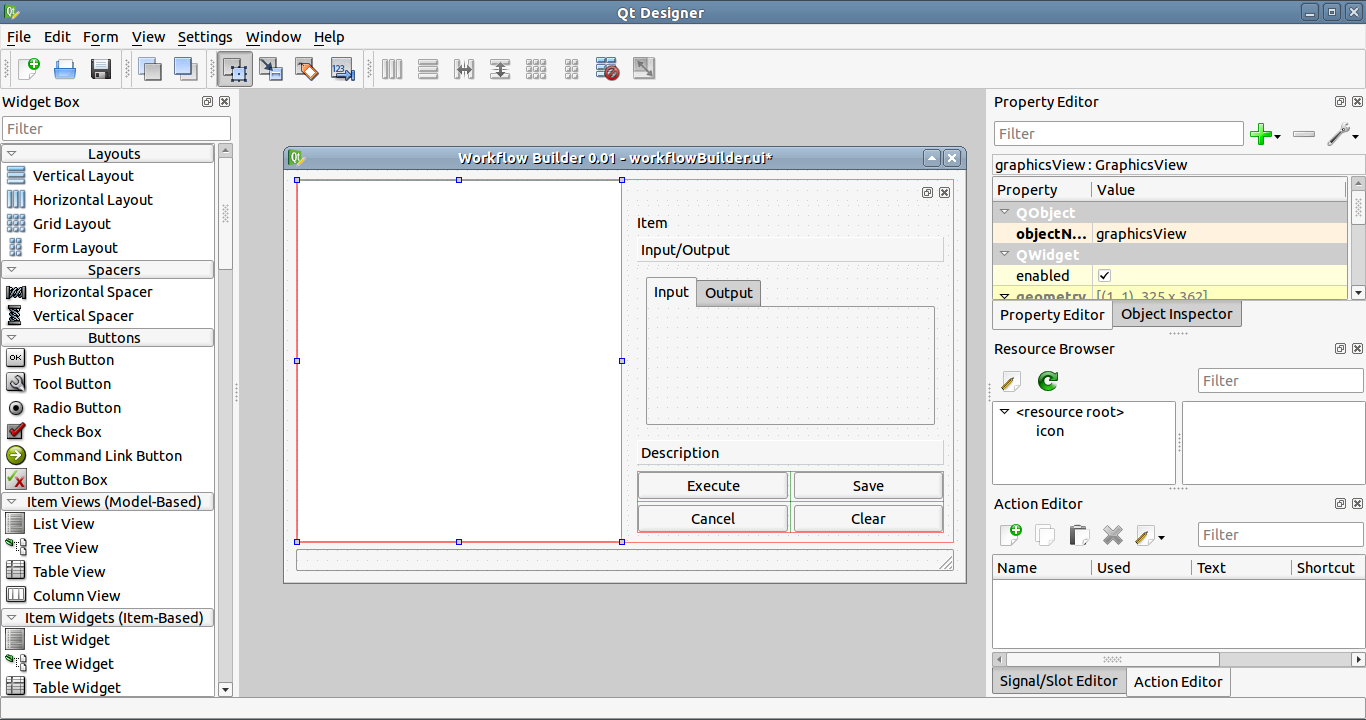
\includegraphics[scale=0.35]{pictures/qt/qt_designer}
	\caption{Qt Designer - nástroj pro tvorbu grafického rozhraní}
  	\label{qtdesigner}
\end{figure}

Soubor vytvořený v Qt Designer (s příponou \textbf{.ui}) lze jednoduše přeložit programem \textbf{pyuic4} do pythoního kódu, který lze poté dále použít. \\

\begin{lstlisting}[label=pyuic4,caption={pyuic4 - přeložení .ui souboru do pythoního kódu}]
		pyuic4 soubor_vytvoreny_v_Qt_Designer.ui -o soubor_v_Pythonu.py 
\end{lstlisting}

%%%%%%%%%%%%%%%%%%%%%%%
%%% Signály a sloty %%%
%%%%%%%%%%%%%%%%%%%%%%%
\newpage
\subsection{Signály a sloty}
Každý objekt knihovny Qt, který je potomkem třídy QObject, má své signály a sloty. Signál je to, co objekt vysílá (emituje), má svůj název. Využívá se při různých změnách objektu. Například když klikneme na objekt \textbf{QPushButton}, vyšle se signál \textit{clicked()}. Tento signál poté můžeme zachytit pomocí metody \textit{connect()}, kterou dědí každý takový objekt knihovny Qt od třídy \textbf{QObject}. Takové propojení signálu a slotu může vypadat například takto \textit{connect($kdoVyslal,SIGNAL("clicked()"), SLOT()$)}. Slot je v podstatě metoda či funkce, která se zavolá na základě nějakého podmětu, signálu. 

Signály a sloty v Qt se hojně využívají při tvorbě grafického rozhraní. Jakékoliv kliknutí, změna textu v \textbf{QLineEdit}, změna prvku v \textbf{QComboBox}, změna pozice grafického objektu ( \textbf{QGraphicsObject} ) či zavření okna vysílají signály. Tyto signály se vysílají bez ohledu, zdali jim nasloucháme či nikoliv. Každá třída má signály a sloty, které dědí po předku, a navíc může obsahovat další, které jsou pro ni typické a mohou se programátorovi hodit. Pakliže nás nějaká změna zajímá, můžeme daný signál zachytit. Kromě toho si můžeme sami napsat svoje vlastní signály či sloty a nemusí se jednat jen o grafické rozhraní. Musíme mít ale na paměti, že objekt, který vysílá signál, musí být potomek objektu \textbf{QObject}. Vyslat signál můžeme  pomocí metody \textit{emit($SIGNAL()$,...)}, kde v $SIGNAL()$ uvedeme název signálu a dále za ním parametry, které se s ním vyšlou. Poté je spojíme se slotem, metodou, která se na jeho základě spustí, pomocí metody $QObject.connect(QObject, SIGNAL, SLOT)$. Tato metoda je statická, tudíž ji můžeme volat přímo z \textbf{QObject}. \\

\noindent Příklad: \\

Předpokládejme, že $tonda$ je objekt třídy \textbf{Tonda}, která je potomkem třídy \textbf{QObject}. Když jde $tonda$ domů, vyšle signál $SIGNAL("jdu")$ s parametrem $"domu"$: \\

%{vyslání slotu s názvem "jdu" s atributem "domu"},morekeywords={Tonda, SIGNAL}

\begin{lstlisting}[label=qtemit,caption={vyslání slotu pod názvem $"jdu"$ s atributem $"domu"$}]
		tonda = Tonda()
		tonda.emit(SIGNAL("jdu"),"domu")
\end{lstlisting}

Marie je také potomek \textbf{QObject} a nachází se kde je jí libo. Marie má v sobě zabudovaný slot a jakmile zachytí signál od $tondy$, že odešel, začne jednat: \\


\begin{lstlisting}[label=qtconnect,caption={zachycení signálu $"odesel"$ od tondy}, morekeywords={Marie, SIGNAL, QObject}]
	class Marie(Object):
		def __init__(self):
			QObject.__init__(self)
			self.connect(tonda, SIGNAL("jdu"), self.jednat)
			# mohou nasledovat dalsi spojeni
		
		def jednat(self, parametr):
			# tady se Marie muze rozhodnout na zaklade parametru, 
			# jak bude jednat
			# napriklad:
			if parametr is "domu":
				self.vecere()
		
	marie = Marie()
\end{lstlisting}

\noindent $tonda$ může emitovat kolik signálů chce a záleží pouze na tom, kolika signálům bude $marie$ naslouchat.

%%%%%%%%%%%%%%%%%%%%%%%%%%%%%%
%%% Model/View Programming %%%
%%%%%%%%%%%%%%%%%%%%%%%%%%%%%%
\subsection{Model-View architektura}
Při seznamování s projektem QGIS Processing Framework a po komunikaci s Camilo Polymeris (student, který začal psát QGIS Processing Framework), jsem začal s přepsáním Processing Manageru (panelu s moduly) z QTreeWidget do MVC architektury. Standardní MVC architektura dělí aplikaci do tří částí, které jsou na sobě co nejméně závislé. Jsou to Model, View a Controller. Oddělení dat od aplikační a prezentační logiky dělá kód přehlednější a lépe udržitelným. Velikou výhodou také je, že jeden model se může zobrazit v několika různých pohledech vždy jiným způsobem.

\begin{figure}[h]
	\centering
	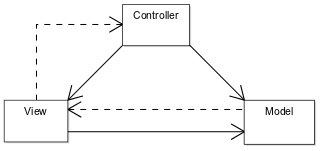
\includegraphics[scale=0.7]{pictures/qt/mvc}
	\caption{Propojení jednotlivých částí architektury MVC}
	\label{mvc}
\end{figure}

\begin{itemize}
	\item{\textbf{Model}} se stará o data - není to pouze místo, kde jsou uložená data, ale jsou zde také definovaná pravidla, kterýma se jednotlivá data řídí
	\item{\textbf{View}} se stará o zobrazení dat v Modelu a o uživatelské rozhraní
	\item{\textbf{Controller}} spravuje reakce na uživatelovi podněty % má na starosti běh událostí, aktualizaci modelu, aplikační logiku
\end{itemize}

V Qt se implementace MVC architektury objevila s verzí Qt4 v podobě model-view-delegate. Kde funkci $controller$u přebírá částečně $view$ (pohled) a částečně $delegate$ (delegát). Delegát určuje, jak budou data editována, případně zobrazena, a komunikuje přímo s pohledem a s modelem. V některých případech může pohled zastávat funkci delegáta. Jedná se o případy, kdy se data editují pomocí jednoduchých editačních nástrojů jako je například editace pomocí \textbf{QLineEdit} u řetězců. Mluvíme tedy o model/view architektuře. Jednoduchý příklad, kde je možné vidět použití hierarchicky uložených dat do modelu a zobrazených ve stromovém pohledu lze najít v \textbf{Příloha 1}. V příkladu je také vidět použití vlastního delegáta a proxy modelu pro vyhledávání mezi daty.

\begin{figure}[h]
	\centering
	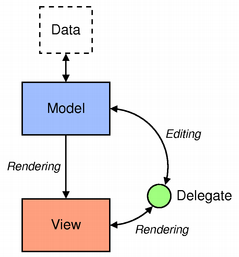
\includegraphics[scale=0.7]{pictures/qt/mv}
	\caption{model-view architektura v Qt4}
	\label{mvc}
\end{figure}

\begin{itemize}
	\item{\textbf{Model}} - tady se nic nemění oproti standardní MVC architektuře; komunikuje se zdrojem dat a poskytuje API pro ostatní komponenty architektury ($view$ a $delegate$)
	\item{\textbf{View}} zobrazuje data a navíc nabízí základní nástroje pro jejich editaci dat
	\item{\textbf{Delegate}} pomocí delegáta můžeme definovat vlastní widgety pro slouží editaci dat a také může definovat, jak se budou jaká data zobrazovat
\end{itemize}

Komunikace mezi jednotlivými komponentami probíhá pomocí signálů a slotů. Qt pro každý prvek architektury ($model$, $view$ a $delegate$) poskytuje základní čistě abstraktní třídy plus několik dalších tříd, již přímo použitelných implementací. Například pro data z tabulky můžeme přímo využít \textbf{QTableModel} a \textbf{QTableView}. Pakliže nám žádná z tříd nevyhovuje, můžeme samozřejmě reimplementovat třídy již existující.

\subsubsection*{Model}
Každý model je založený na abstraktní třídě \textbf{QAbstractItemModel}. Pakliže budeme chtít zobrazovat data jako seznam či v tabulce můžeme se poohlídnout po dalších abstraktních třídách \textbf{QAbstractListModel}, resp. \textbf{QAbstractTableModel} implementující další prvky, které jsou pro daný model typické. Jak je již z názvu vidno, žádná z těchto tříd nemůže být použita přímo. Mohou nám posloužit k napsání svých vlastních modelů. Také se můžeme pokusit vybrat si z několika základních modelů, které jsou připraveny k přímému použití. Mezi tyto modely patří například \textbf{QStringListModel} pro seznamy řetězců a \textbf{QStandardModel} pro složitější data. Dále existují typy určené pro přístup do databází (\textbf{QSqlQueryModel}, \textbf{QSqlTableModel} a \textbf{QSqlRelationalTableModel}) či \textbf{QFileSystemModel}, který poskytuje informace o souborech a složkách na vašem lokálním souborovém systému. Máme tedy několik předpřipravených modelů. Nebudou-li nám ale plně vyhovovat, můžeme si kterýkoliv vybrat a reimplementovat jej.

Dále existují tzv. proxy modely, které stojí mezi view a "standardním" modelem a poskytují podporu pro zpracování dat.  Například \textbf{QSortFilterProxyModel}, který umožňuje uživateli vytvořit pravidla pro řazení a filtraci dat.

View a Delegate získávají a manipulují s daty uloženými v modelech pomocí indexů třídy \textbf{QModuleIndex} a rolí. Index nám udává pozici v modelu pomocí rodiče, řádku a sloupce. V indexu mohou být uložena různá data pomocí různých rolí.

\begin{figure}[h]
	\centering
	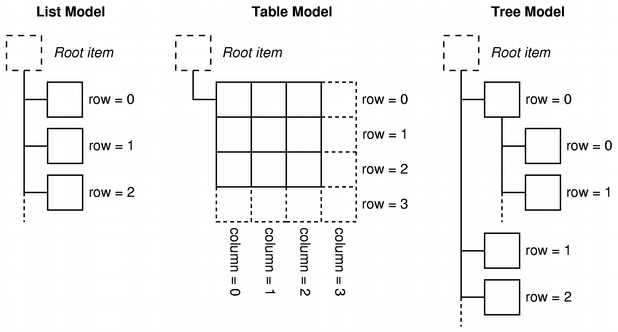
\includegraphics[scale=0.7]{pictures/qt/mv_models}
	\caption{modely v model-view architektuře a jejich pozicování}
	\label{mvModels}
\end{figure} 

\begin{table}[h]
	\centering
	\begin{tabular}{|c|c|}
		\hline	
		metoda & popis \\
		\hline
		\hline
		child(int row, int column) & vrací potomka na dané pozici QModelIndex \\
		\hline
		data(int role) & vrací data v podobě QVariant \\
		\hline
		model() & vrací model, ve kterém se nachází daný index \\
		\hline
		parent() & vrací rodiče v podobě QModelIndex \\
		\hline
	 	\multirow{2}{*}{row(), column()} & vrací číslo sloupce/řádku daného \\ 
		 & indexu vůči jeho rodiči \\
		\hline
	\end{tabular}
	\caption{některé metody třídy QModelIndex}
	\label{tab:qmodelindex}
\end{table}

\textit{role} je celé číslo, na základě kterého můžeme zjistit "roli" dat. Existuje několik základních rolí jako $DisplayRole$(0), $ToolTipRole$(3) či $UserRole$(32). Samozřejmě si můžeme v podstatě zvolit jakékoliv celé číslo. Zde se s oblibou využívá $UserRole$, která reprezentuje nejvyšší číslo z předdefinovaných rolí (například $UserRole$ + celé číslo). Z QModelIndex dostaneme data pomocí metody $data(role)$.

Obecně se data do modelu ukládají pomocí metody $setData$( QModelIndex index, QVariant value, int role ). Z objektu QVariant můžeme dostat naše data voláním metod jako $toInt()$, $toString()$, $toRect()$... řípadně $toPyObject()$ [v ukázce \ref{qstandarditem}]. 


\begin{table}	
	\centering
	\begin{tabular}{|c|c|}
		\hline	
		metoda & popis \\
		\hline
		\hline
		data(QModelIndex index, int role) & vrací data v podobě QVariant \\
		\hline
		setData(QModelIndex index, QVariant value, int role) & uloží data do modelu \\
		\hline
		insertRow(int row, QModelIndex parent) & vloží data na danou pozici \\
		\hline
		removeRow(int row, QModelIndex parent) & maže data na dané pozice \\
		\hline
		index(int row, int column, QModelIndex parent) & vrací index na dané pozici \\
		\hline


	\end{tabular}
	\caption{některé metody třídy QAbstractItemModel}
	\label{tab:qabsmodel}
\end{table}

U modelu \textbf{QStandardItemModel} se může k položkám v modelu přistupovat také jako \textbf{QStandardItem}. Data se do modelu ukládají jako \textbf{QStandardItem()} objekt. Pro uložení informací do objektu \textbf{QStandardItem} se používá metoda $setData$(QVariant \textit{data}, int \textit{role}). Pakliže nastavíme data pouze pomocí $setData$(\textit{data}), role se nastaví na $UserRole + 1$. Data potom dostaneme s \textbf{QStandardItem} pomocí metody $data(role)$. Model s QStandardItemModel s QStandardItem se hodí pro hierarchicky uspořádaná data. [ukázka použití QStandardItem \ref{qstandarditem} \\

\begin{lstlisting}[label=qstandarditem,caption={QStandardItem - vytvoření a získání dat}, morekeywords={PyQt4, QtCore, QtGui, QStandardItem, Qt, Qt.UserRole, Qt.DisplayRole}]
	from PyQt4.QtCore import Qt
	from PyQt4.QtGui import QStandardItem

	student = QStandardItem("Tonda")
	student.setData(24)
	student.setData("Geoinformatika", Qt.UserRole + 2)

	# vytiskne (24, True) - True znamena, ze se jedna o cislo
	print student.data().toInt() 					
	# vytiskne (24, True)
	print student.data(Qt.UserRole + 1).toInt()		
	# vytiskne "Tonda"
	print student.data(Qt.DisplayRole).toString() 	
	# vytiskne "Geoinformatika"
	print student.data(Qt.UserRole + 2).toString() 	

\end{lstlisting}

Obecně tedy data ukládáme pomocí metody $setData$ a získáváme pomocí $data$. Kde na stejnou pozici můžeme uložit více dat s různými rolemi.
 
\subsubsection*{View}

Pomocí pohledů Qt umožňuje zobrazovat data uložená v modelu. Jeden model můžeme zobrazovat v několika různých pohledech. Všechny pohledy jsou potomky abstraktní třídy \textbf{QAbstractItemView}, ta je potomek třídy QAbstractScrollArea a přes QFrame se dostaneme ke třídě \textbf{QWidget}. S pohledy tedy můžeme zacházet jako s ostatními widgety. Model se do view nastaví pomocí metody $setModel$( QAbstractItemModel model). Jednotlivé prvky z modelu jsou pohledu dostupné opět pomocí indexů (QModelIndex). Pohled dokáže prvky zobrazit, řekněme, obyčejně. Pakliže si chceme se zobrazením prvků pohrát více (například měnit font či barvu podle nějakých vlastností dat), použijeme k tomu delegáta. Ten se se nastaví pomocí metody $setItemDelegate$(QAbstractItemDelegate delagate). [ukázka viz \ref{qview}] \\

\begin{lstlisting}[label=qview,caption={View - vytvoření pohledu a nastavení modelu a delegáta}, morekeywords={QItemDelegate, QStandardItemModel, QTreeView}]
	model = QStandardItemModel()
	delegate = QItemDelegate()

	view = QTreeView()
	view.setModel(model)
	view.setItemDelegate(delegate)
\end{lstlisting}

Pro data, která budou zobrazována jako seznam, můžeme využít pohled \textbf{QListView}, pro tabulková data \textbf{QTableView}, pro stromová data pak \textbf{QTreeView}.

\subsubsection*{Delegate}
Všichni delegáti musí být potomky abstraktní třídy \textbf{QAbstractItemDelegate}. Qt nám nabízí k přímému použití třídy QItemDelegate a QStyledItemDelegate. $View$ má defalutně nastaveného delegáta QStyledItemDelegate. Pomocí delegáta můžeme určit, jak se budou dané položky z modelu zobrazovat a jak se budou editovat. 

Pakliže máme v modelu například jako data uloženy studenty a chceme, aby byli vypisováni studenti modře a studentky červeně můžeme si vytvořit vlastního delegáta, který nám to umožní. V tomto případě [ukázka kódu \ref{qdelegate}] využijeme QStyledItemDelegate a přepíšeme metodu $paint$ například takto: \\

\begin{lstlisting}[label=qdelegate:paint,caption={Delegate - přepsání metody $paint$}, morekeywords={QItemDelegate, Qt, QFont, AlignLeft, DisplayRole, UserRole, QPen}]
class Delegate(QItemDelegate):
    def __init__(self, parent=None, *args):
        QItemDelegate.__init__(self, parent, *args)

    def paint(self, painter, option, index):
        painter.save()       
        
        # nastaveni fontu
        painter.setPen(QPen(Qt.black))
        painter.setFont(QFont("Times", 10, QFont.Bold))
        
		# nastaveni barvy podle pohlavi
        if index.data(Qt.UserRole + 3).toString() == "female":
            painter.setPen(QPen(Qt.red))
        elif index.data(Qt.UserRole + 3).toString() == "male":
            painter.setPen(QPen(Qt.blue))

        value = index.data(Qt.DisplayRole)
        if value.isValid():
            text = value.toString()
            painter.drawText(option.rect, Qt.AlignLeft, text)
            
        painter.restore()
\end{lstlisting}

        
\noindent V tomto příkladě \ref{qdelegate:paint} předpokládáme, že data (v podobě indexů) obsahují informaci o pohlaví uloženou pod rolí $Qt.UserRole + 3$.

Editor (widget pro editaci dat) nastavíme reimplementací metody $createEditor$, která vrací QWidget. Aby se po editaci změnila data v modelu, musíme také reimplementovat metodu $setModelData$. V ukázce kódu \ref{qdelegate:createEditor} předpokládáme, že třída $editStud$ je widget, který je složen z dvou dalších widgetů - QLineEdit pro editaci jména a QSpinBox pro nastavení věku. \\

\begin{lstlisting}[label=qdelegate:createEditor,caption={Delegate - přepsání metod $createEditor$ a $setModelData$}, morekeywords={QItemDelegate, Qt, QFont, AlignLeft, DisplayRole, UserRole, QPen}]
class Delegate(QItemDelegate):
    def __init__(self, parent=None):
        QItemDelegate.__init__(self, parent)
    def createEditor(self, parent, option, index):
    	# editStud je widget slozeny z QLineEdit a QSpinBox
        editor = editStud(index, parent)
        return editor    
    def setModelData(self, editor, model, index):
        model.setData(index,QVariant(editor.name()))
        model.setData(index,QVariant(editor.age()), Qt.UserRole+4)
\end{lstlisting}

Použití QStandardItemModel s QTreeView za použití proxy modelu a delegáta z ukázek \ref{qdelegate:paint} a \ref{qdelegate:createEditor} můžeme dostat výsledek podobný tomuto:

\begin{figure}[h]
	\centering
	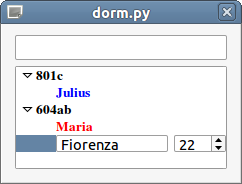
\includegraphics[scale=0.7]{pictures/qt/dorm}
	\caption{Ukázka použití QStandardItemModel, QTreeView, delegáta a proxy modelu.}
	\label{pic:delegate}
\end{figure} 

\noindent
V horní části vidíme widget QLineEdit, která je propojený s proxy modelem a slouží s vyhledávání v datech. Barevně odlišené pohlaví je způsobené delegátem, stejně jako řádek, který se edituje (QLineEdit + QSpinBox). Celý příklad najdete v příloze.

%%%%%%%%%%%%%%%%%%%%%
%%% Drag and Drop %%%
%%%%%%%%%%%%%%%%%%%%%
\subsection{Drag and Drop}
Zjednodušeně řečeno Drag and Drop je mechanismus, který nám umožňuje vzít jeden objekt z jednoho místa a přesunout ho na druhé. A to nejen v rámci jedné aplikace, ale také mezi různými aplikacemi. Na základě 'dopadu' (drop) objektu můžeme vyvolávat různé akce. Můžeme definovat, který objekt může být přetahován nebo které objekty mohou dopadnout na daný objekt (které objekty budou akceptovány). Data se přenáší pomocí objektu \textbf{QDrag}, do kterého se uloží data v podobě \textbf{QMimeData}.

Pro umožnění chytnutí objektu (widgetu) myší, přepíšeme metodu $mouseMoveEvent$, která je děděna z \textbf{QWidget}. Zde můžeme nastavit, které tlačítko myši budeme akceptovat a další pravidla na základě kterých se vytvoří či nevytvoří objekt třídy \textbf{QDrag}. 

Akceptování dopadnutých objektů, nastavíme metodou $acceptDrops$ s parametrem True. Dále musíme přepsat metodu $dragEnterEvent$(event), $dragMoveEvent$(event) a $dropEvent$(event), kde akceptujeme event (událost) pomocí metody její $accept$(). Jednotlivé události jsou objekty tříd \textbf{QDragEnterEvent}, \textbf{QDragMoveEvent} a \textbf{QDropEvent}. Třída \textbf{QDropEvent} obsahuje metodu $source$(), která nám vrací zdrojový widget \textbf{QDrag} objektu. Pomocí toho se také můžeme rozhodnout, zda danou událost příjmem či nikoliv.

Tohoto mechanismu jsem využil při přetahování modulů z Processing Manageru do Workflow Builderu. Dále toho také využívá Graphics View Framework při pohybu grafických prvků.

%%%%%%%%%%%%%%%%%%%%%%%%%%%%%%%
%%% Graphics View Framework %%%
%%%%%%%%%%%%%%%%%%%%%%%%%%%%%%%
\subsection{Graphics View Framework}
Graphics View Framework nabízí prostředí pro práci s velkým počtem grafických dvojrozměrných prvků. Nabízí také widget, ve kterém se dané prvky zobrazují. Podporuje funkce jako zoom nebo rotaci. Prostředí umožňuje spravovat klasické události jako kliknutí myši, její pohyb či stisknutí klávesy. 

Prostředí staví, podobně jako model-view architektura, na principu, kdy jsou samotná data oddělena od způsoby jejich zobrazení. V Graphics View Framework nahrazuje model scénou (\textbf{QGraphicsScene}) a pohled zastupuje \textbf{QGraphicsView}. Základní třídou grafických prvků je \textbf{QGraphicsItem}. Z této třídy poté dědí několik dalších jejich reimplementací jako QGraphicsRectItem, QGraphicsPathItem či QGraphicsSimpleTextItem. 

\subsubsection*{QGraphicsItem}
QGraphicsItem je základní třída, ze které vychází ostatní grafické 2D prvky. Pomocí metody setPos se nastaví pozice v rodiči. Pakliže žádný rodič není, bere se pozice ve scéně (QGraphicsScene). V Graphics View Framework také funguje hierarchie. Prvkům můžeme nastavit rodiče buď při jejich vytváření, či pomocí metody $setParentItem$(QGraphicsItem parent). Prvkům můžeme nastavit různé vlastnosti například jak budou graficky vypadat či zdali mohou být přesouvány. Mezi standardní grafické prvky, které reprezentují klasické tvary, patří:\\

\begin{itemize}
	\item QGraphicsRectItem
	\item QGraphicsPathItem
	\item QGraphicsLineItem
	\item QGraphicsPolygonItem
	\item \ldots
\end{itemize}
 
Prvkům můžeme dále nastavovat tzv.ToolTip pomocí metody $setToolTip$(QString toolTip) či tzv. flagy pomocí $setFlag$(GraphicsItemFlag flag, bool enabled = true) a $setFlags$(GraphicsItemFlags flags). Flagy slouží k nastavení chování prvku. Například chceme-li s prvkem pohybovat, nastavíme flagy QGraphicsItem.ItemIsMovable, QGraphicsItem.ItemIsSelectable a QGraphicsItem.ItemIsFocusable na hodnotu true [viz ukázka kódu \ref{qgraphicsitem:flags}].\\
 
\begin{lstlisting}[label=qgraphicsitem:flags,caption={Nastavení flagů u QGraphicsRectItem}, morekeywords={QGraphicsItem, QGraphicsRectItem}] 
	rect = QGraphicsRectItem()
	rect.setFlags(QGraphicsItem.ItemIsMovable | \
				  QGraphicsItem.ItemIsSelectable | \
				  QGraphicsItem.ItemIsFocusable)
\end{lstlisting}
 
\subsubsection*{QGraphicsScene}
Do scény se prvky přidávají pomocí metody $addItem$(QGraphicsItem item) a mažou se ze scény pomocí $removeItem$(QGraphicsItem item). Pro smazání všech prvků ve scéně použijeme metodu $clear$(). Další užitečné metody jsou například $items$(), která nám vrací všechny prvky scény, $itemAt$(QPointF point), která nám vrací prvek na vybrané pozici, či $selectedItems$(), která nám vrací seznam vybraných prvků.

\subsubsection*{QGraphicsView}
U QGraphicsView nastavíme scénu pomocí setScene(). Dále může nastavit možnost přibližování a oddalování, měřítko, barvu pozadí, vyhlazování hran u prvků, můžeme rotovat scénu atp.

Na obrázku je vidět jedna scéna zobrazena ve dvou rozdílných pohledech. Změna scény provedená v jednom pohledu, se projeví také v druhém pohledu.

\begin{figure}[h]
	\centering
	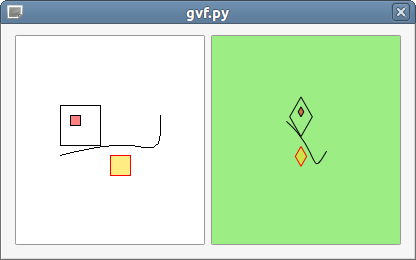
\includegraphics[scale=0.7]{pictures/qt/gsf}
	\caption{Zobrazení jedné scény ve dvou různých pohledech.}
	\label{gsf}
\end{figure}


\subsection{VisTrails, Orange}
Na začátku práce na Workflow Builderu se nabízela možnost využít některých svobodných projektů pro modelování workflow diagramů. Vzhledem k tomu, že QGIS využívá knihovnu Qt a QGIS Processing framework samotný je psaný  v Pythonu, naskýtali se jako možnosti inspirace projekty Orange či VisTrails.

Nakonec mě nejvíce oslovilo grafické zpracování VisTrails. Uživatel na první pohled vidí, který parametr je s kterým spojen. Ne pouze který modul je s kterým spojen jak to často bývá u podobných programů. Jal jsem se tedy studovat kód a využil jsem prvky scény QGraphicsModule, QGraphicsPort a QGraphicsConnection.

Obrazek

%VisTrails is a scientific workflow management system developed at the Scientific Computing and Imaging Institute at the University of Utah that provides support for data exploration and visualization. It is written in Python and employs Qt via PyQt bindings. The system is open source, released under the GPL v2 license. The pre-compiled versions for Windows, Mac OS X, and Linux come with an installer and several packages, including VTK, matplotlib, and ImageMagick. VisTrails also supports user-defined packages.
\newpage
\index{QGIS Processing Framework}
\section{QGIS Processing Framework}
\nocite{pf:www}


\begin{center}
		
\includegraphics[scale=0.30]{pictures/qgis_pf}
\end{center}

QGIS Processing Framework vznikl v rámci projektu GSoC
2011\footnote{Google Summer of Code. Projekt společnosti Google
na podporu studentu, více na \url{http://code.google.com/soc/}}. Student
Camilo Polymeris z univerzity Universidad de Concepción si kladl za
cíl napsat obecný framework, do kterého budou zapadat všechny moduly
všech pluginů QGISu a každý modul bude možné použít buď samostatně
nebo spojovat s jinými.

V době psaní této práce byla na světě první verze Processing
Frameworku a vše nasvědčovalo tomu, že práce na frameworku budou
pokračovat a nástroje v Processing Frameworku budou
přibývat. Existovala totiž pouze částečná podpora pro funkce SAGA
GIS a plugin zpřístupňující funkce \index{Orfeo Toolbox, OTB} Orfeo
Toolboxu (OTB). Orfeo Toolbox je svobodný software poskytující
nástroje pro zpracování snímku z \index{DPZ, dálkový průzkum Země}
dálkového průzkumu Země.

V době mého připojení k QGIS Processing Frameworku byl projekt na
začátku. Pro seznámení s projektem jsem přepsal Processing Manager
(toolbox) z QTreeWidget do MVC architektury.

\begin{figure}[h]
	\centering
	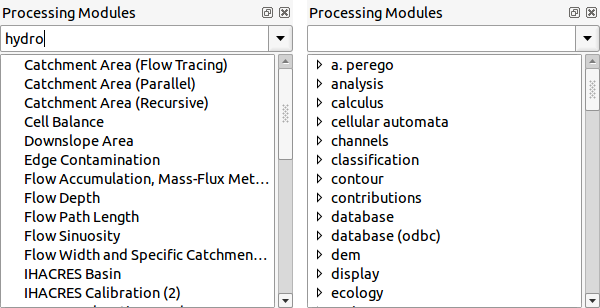
\includegraphics[scale=0.5]{pictures/pf/processing_manager_small}
	\caption{QGIS Processing Framework - Processing Manager}
  	\label{pf:pm}
\end{figure}

Processing Manager je část QGIS Processing Frameworku, která
zpřístupňuje všechny moduly dostupné skrze QGIS Processing Framework z
jednoho místa. Jedná se o panel se seznamem modulů, které jsou
rozděleny podle tagů do různých skupin (například 'raster',
'hydrology'). Každý modul obsahuje seznam tagů, které napovídají, k
čemu daný modul slouží. Uživatel může najít hledaný modul
prohledáváním samotného stromu, či využít vyhledávací okénko v horní
části panelu. Processing Manager prohledává tagy daného modulu a jeho
název. Modul obsahuje dále popis, ale protože se tagy generují z
tohoto popisu, není nutné popis procházet \figurename \ref{pf:pm}.

Modul je reprezentován třídou \textbf{Module} a jeho instance
třídou \textbf{ModuleInstace}. Z~třídy \textbf{Module} získáváme
informace o modulu. Pomocí metody $name$() získáme jméno modulu,
metoda $description$() vrací popis, metoda $tags$() a metoda
$instance$() vrací instanci třídy \textbf{ModuleInstace} daného
modulu. Zavoláním metody $parameters$() získáme seznam parametrů
daného modulu. Parametry jsou třídy \textbf{Parameter}.

U \textbf{ModuleInstace} můžeme pomocí metody $setValue$(Parameter,
hodnota) přiřazovat parametrům konkrétní hodnoty. Metodou
$value$(Paramter) získáme hodnotu parametru. Pomocí metody
$setState$() s parametrem "2"\,spouštíme daný modul. Metoda $module$()
vrací module (Module).

Parametry jsou třídy \textbf{Parameter}. Uchovávají v sobě informaci o
názvu a popisu parametru, zdali je parametr povinný, jakého je typu a
role (např. vstupní, výstupní) a jeho defaultní hodnotu. Přehled metod
třídy \textbf{Parameter} je zobrazen v [\tablename \ref{tab:metPar}].

\begin{table}[!]
	\centering
	\begin{tabular}{|c|c|}
	\hline
	{\bf metoda} & {\bf popis} \\
	\hline
	\hline
	name() & vrací jméno\\
	description() & vrací popis\\
	type() & vrací typ [viz Tabulka \ref{tab:pf_parametry} \\
	setRole(role) & nastaví roli\\
	role() & vrací roli\\
	setMandatory(bool) & nastaví zdali je parametr povinný\\
	isMandatory() & vrátí hodnotu, zdali je parametr povinný\\
	setDefaultValue() & nastaví defaultní hodnotu parametru\\
	defaultValue() & vrátí defaultní hodnotu parametru \\
	\hline
	\end{tabular}
	\caption{Metody třídy Parameter.}
	\label{tab:metPar}
\end{table}

Modulů z \textbf{QGIS Processing Framework} jsou přístupné buď přes \textbf{Processing Manager} nebo přes pythoní konzoli [\autoref{pf:konzole}]. Konzoli lze spustit například klávesovou zkratkou \textbf{Ctrl+Alt+ p}. 
\newpage

\begin{lstlisting}[label=pf:konzole,caption={Přístup k modulům přes konzoli.}] 
import processing

# seznam vsech registrovanych modulu
processing.framework.modules()
	
# vrati dany modulu
mod = processing.framework['nazev_modulu']
# vraci seznam parametru daneho modulu
mod.parameters()

# vytvori instanci modulu
instance = mod.instance()
# nastavi paramter
instance.setValue(parametr, hodnota)
# spusti modul
instance.setState(2)

# ziskani hodnoty parametru
instance.value(parametr2)
\end{lstlisting}

Spouští-li se modul přes \textbf{Processing Manager}, objeví se
dialogové okno pro nastavení parametrů modulu a následné spuštění
[viz \figurename \ref{pf:dialog}].

\begin{figure}[!]
	\centering
	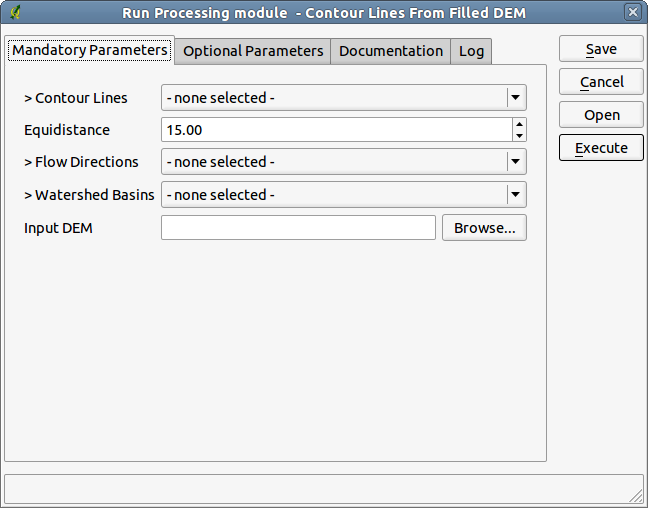
\includegraphics[scale=0.5]{pictures/pf/processing_dialog}
	\caption{QGIS Processing Framework - okno pro nastavení a spuštění modulu}
  	\label{pf:dialog}
\end{figure}

%%%%%%%%%%%%%%%%%%%
%%% SAGA Plugin %%%
%%%%%%%%%%%%%%%%%%%
\newpage
\subsection{SAGA Plugin}
SAGA Plugin vznikl v rámci stejného projektu Camila Polymeris pro GSoC
2011. Měl zpřístupňovat funkce programu SAGA GIS pomocí jeho API
uživatelům Quantum GIS. Na stránkách
projektu \cite{pf:supportedModules} se deklaruje, že by mělo být
podporováno 170 modulů z celkových 425. Toto číslo vychází z
předpokladu, že moduly, u kterých jsou všechny vstupní i výstupní
parametry podporovány, pracují správně. Podporované parametry SAGA GIS
a jejich reprezentace v Processing
Frameworku \ref{tab:saga_parameters}. Parametry SAGA GIS, které nejsou
podporované Processing Frameworkem$:$ \textit{Table field, Data
Object, Grid list, Table, Node, Shape list, Parameters, Point Cloud,
TIN, Static table, Table list, Color, TIN list a Colors}. Dále nejsou
podporované interaktivní moduly. Bohužel ale nebyl plugin plně
dokončen a skutečný počet správně pracujících pluginů není roven
170. \\

\begin{table}[h]
	\centering
	\begin{tabular}{|c|c|}
		\hline
		\textbf{SAGA parametr} & \textbf{PF Parameter} \\
		\hline
		\hline
		Int & \multirow{3}{*}{NumericParameter}\\
		Double & \\
		Degree & \\
		\hline				
		Range & RangeParameter\\	
		\hline
		Bool & BooleanParameter\\		
		\hline
		String & \multirow{2}{*}{StringParameter}\\
		Text & \\
		\hline
		Chioce & ChoiceParameter\\
		\hline
		FilePath & PathParameter\\
		\hline
		Shapes & VectorLayerParameter\\
		\hline
		Grid & RasterLayerParameter\\		
		\hline	
	\end{tabular}
	\caption{parametry SAGA GIS podporované Processing Frameworkem}
	\label{tab:saga_parameters}
\end{table}


%%%%%%%%%%%%%%%%%%%%%%%%%%%%
%%% Psaní pluginu pro PF %%%
%%%%%%%%%%%%%%%%%%%%%%%%%%%%

\subsection{Psaní pluginu pro PF}
Plugin pro QGIS Processing Framework se v mnohém neliší od normálních
pluginů psaných pro QGIS. Inicializační soubor se prakticky vůbec
neliší. Třída reprezentující samotný plugin obsahuje navíc
metodu \textit{modules}(), která vrací seznam modulů třídy
processing. \textbf{Module} (dále jen Module), který poskytuje daný
plugin. Plugin samotný se musí registrovat v frameworku. To se provede
příkazem \begin{scriptsize}processing.framework.registerModule\-Provider(self)\end{scriptsize},
který se vloží do metody \textit{initGUI}().

Plugin tedy může obsahovat několik modulů, které vrací pomocí
metody \textit{modules}(). Každý modul se skládá ze sebe a ze svojí
"instance". Tedy z podtříd tříd Module a processing.ModuleInstance
(dále jen ModuleInstance). Module je pro daný modul základní třída,
která definuje typy parametry modulu, jeho název, popis a tagy. A
vrací jeho instanci v podobě ModuleInstance, která slouží ke spouštění
modulu s nastavenými parametry a spravuje, co se děje po provedení
modulu. To znamená, že pakliže chceme spustit modul, musíme nastavit
parametry a ty se nastavují v instanci, ne v~modulu samotném. Modul
poté spustíme metodou instance setStatus(2). Instance by mela
obsahovat kód, který vstupní parametry zpracuje a poté také nastaví
výstupní hodnoty.

Modul může mít několik vstupních a výstupních parametrů. V současné
době dovoluje framework uživateli použít
parametry \ref{tab:pf_parametry}.

\begin{table}	
	\centering
	\begin{tabular}{|c|c|c|}
		\hline
		\textbf{parametr} & \textbf{popis} & \textbf{grafická reprezentace}\\
		\hline
		\hline
		NumericParameter & číslo & QSpinBox\\
		\hline
		RangeParameter & dvojice číselných hodnot & pár QSpinBox\\	
		\hline
		BooleanParameter & boolean & QCheckBox\\		
		\hline
		\multirow{2}{*}{ChoiceParameter} & seznam možností & \multirow{2}{*}{QComboBox}\\
		& např. vrstev, metod & \\
		\hline
		StringParameter & textový řetězec & QLineEdit \\
		\hline
		PathParameter & cesta k souboru & QLineEdit + QPushButton \\
		\hline
		\multirow{2}{*}{VectorLayerParameter} & \multirow{2}{*}{QgsVectorLayer} & QComboBox s registrovanými \\
		& & vektorovými vrstvami\\
		\hline
		\multirow{2}{*}{RasterLayerParameter} & \multirow{2}{*}{QgsRasterLayer} & QComboBox s registrovanými \\
		& & rastrovými vrstvami\\		
		\hline	
	\end{tabular}
	\caption{parametry podporované Processing Frameworkem}
	\label{tab:pf_parametry}
\end{table}

Jako příklad uvedeme plugin Plugin, který bude mít na vstupu dva
parametry. Jeden parametr pro načtení cesty k rastrovému souboru a
druhý pro zadání jeho názvu, pod kterým se objeví v QGISu. Výstup bude
jeden - rastr třídy QgsRasterMapLayer. Příklad je pouze ilustrativní.

Inicializační soubor nebudu uvádět, protože se nijak neliší od toho,
když píšeme normální plugin pro QGIS. Soubor se samotným pluginem bude
obsahovat třídu Plugin, která reprezentuje náš plugin
[\autoref{pf:plugin}]. Dále třídu RasterToQgis(processing.\-Module)
[\autoref{pf:rasterToQgis}] a třídu
RasterToQgisInstance(processing.ModuleInstance)
[\autoref{pf:rasterToQgisInstance}].\\

\newpage
\begin{lstlisting}[caption={Třída Plugin pro QGIS Processing Framework}, label=pf:plugin, morekeywords={Plugin, __init__, modules, initGUI, unload}]
class Plugin:
    def __init__(self, iface):
        self.iface = iface
    def unload(self):
        pass
    def modules(self):
        return [self.rasterInputLayer]
    def initGui(self):
        self.rasterInputLayer = RasterToQgis(self.iface)
        processing.framework.registerModuleProvider(self)
\end{lstlisting}
\newpage
\begin{lstlisting}[caption={Třída RasterToQgis reprezentující modul pro QGIS Processing Framework}, label=pf:rasterToQgis, morekeywords={processing.Module,RasterToQgis, __init__, instance, RasterToQgisInstance, PathParameter, StringParameter, RasterLayerParameter}]
class RasterToQgis(processing.Module):
    def __init__(self, iface = None):
        self.iface = iface
        self.inParamPath = PathParameter("Path to input raster",
        	role=Parameter.Role.input)
        self.inParamName = StringParameter("Name of layerr",
        	role=Parameter.Role.input)
        self.outParam = RasterLayerParameter("Output raster",
        	role = Parameter.Role.output)
        self.outParam.setMandatory(False)
        processing.Module.__init__(self, "Input raster by path", 
            description = "Description",
            parameters = [self.inParamPath,self.inParamName,self.outParam], 
            tags = ["raster", "input"])

    def instance(self):
        return RasterToQgisInstance(self, self.inParamPath,
        							self.inParamName,  self.outParam)
\end{lstlisting}

V příkladu [\autoref{pf:rasterToQgis}] jsme u parametrů nastavili
pouze nejnutnější atributy jako název a roli. Role nám říká, zdali je
parametr povinný či volitelný. U parametrů můžeme nastavit také popis
či počáteční hodnotu při jejich tvorbě pomocí parametrů v
konstruktoru \textit{description} a \textit{defaultValue}. Nastavit
defaultní hodnotu můžeme také
metodou \textit{setDefaultValue}(value). \\

\begin{lstlisting}[caption={Třída RasterToQgisInstance reprezentující instanci modulu pro QGIS Processing Framework}, label=pf:rasterToQgisInstance, morekeywords={processing.ModuleInstance, RasterToQgisInstance, __init__, valueChangedSignal,onStateParameterChanged, QgsRasterLayer,setValue }]
class RasterToQgisInstance(processing.ModuleInstance):
    def __init__(self, module, inParamPath, inParamName,  outParam):
        self.inParamPath = inParamPath
        self.inParamName = inParamName
        self.outParam = outParam
        processing.ModuleInstance.__init__(self, module)
        QObject.connect(self,
            self.valueChangedSignal(self.stateParameter),
            self.onStateParameterChanged)
    def onStateParameterChanged(self, state):
        if state == StateParameter.State.running:            
            path = self[self.inParamPath]
            name = self[self.inParamName]
            raster = QgsRasterLayer(path, name)
            self.setValue(self.outParam, raster)
            self.setState(StateParameter.State.stopped)
\end{lstlisting}

Instance kontroluje stav (state) modulu. Je-li nastaven hodnotu 2
(StateParameter.State.running) vezme si vstupní parametry a na jejich
základě vytvoří novou rastrovou vrstvu \textbf{QgsRasterLayer}. A tu
nastaví do odpovídajícího výstupního parametru.

%%%%%%%%%%%%%%%%%%
%%% Conclusion %%%
%%%%%%%%%%%%%%%%%%

\subsection{Závěr}

Bylo by dobré vyřešit vstupní vrstvy aby například rastrová vrstva
zadaná jako PathParameter byla kompatibilní s parametrem
RasterLayerParameter. Dát vývojáři pluginu možnost, aby mohl uživatel
zadat vrstvu buď pomocí cesty nebo výběrem z již načtených vrstev. Dát
tedy uživateli obě možnosti.

Do této chvíle je napsán OTB Plugin pro zpracování družicových snímků
a rozepsán SAGA Plugin s podporou několika pluginů z SAGA GIS.

Camilo Polymeris měl v plánu pokračovat na projektu v rámci GSoC 2012,
ale po objevení frameworku SEXTANTE svoji žádost stáhl a zapojil se do
prací na SEXTANTE. QGIS Processing Framework se tedy zdá být mrtvým
projektem.

Dále bych chtěl upozornit, že během vývoje se změnila struktura
dat. Na začátku bylo jádro frameworku uloženo
v \begin{scriptsize}python/processing\end{scriptsize} a Processing
Manager, GUI a dialog pro spouštění modulů
v \begin{scriptsize}python/plugins/processingplugin\end{scriptsize}. V
současné době je vše uloženo
v \begin{scriptsize}python/processingmanager\end{scriptsize},
resp. jádro
v \begin{scriptsize}python/processingmanager/processing\end{scriptsize}. To
může na začátku psaní vlastního pluginu způsobit menší problém v
chybně zadané cestě k frameworku.

\newpage

\newpage

\section{xml.dom.monidom}
\nocite{python:www}
\nocite{py3:book}

Nově vzniklé workflow se ukládají do souboru využívajíce
jazyk \index{XML} XML. Výhoda XML dokumentu je, že se s ním snadno
pracuje a jde v podstatě pouze o textový dokument.

XML nabízí jednoduché uložení hierarchicky strukturovaných dat. O
prvcích XML dokumentu hovoříme jako o elementech. Elementy jsou
ohraničeny počátečními a koncovými znaky, tzv. tagy. XML dokument
obsahuje vždy právě jeden kořenový element, který se může skládat z
dalších a dalších elementů. V příkladu XML dokumentu
(\autoref{xml:example}]) je kořenový element $Graph$. Elementy mohou
obsahovat atributy (dvojice jméno="hodnota").  Jména atributů se v
rámci jednoho elementu nesmí opakovat. Elementy také mohou obsahovat
text, který se uvádí mezi počátečním a koncovým znakem. \\

\noindent Příklad XML dokumentu$:$ \\

\lstinputlisting[language=XML,caption={Příklad XML dokumentu},morekeywords={Graph, SubGraph, Module, tag}, label=xml:example]{code/plugins/xml/example_xml.xml}

% DOM level 2
Pro práci s XML dokumenty se v prostředí jazyka Python nabízí několik
modulů. Při psaní této práce byl
vybrán \index{xml.dom} \textbf{xml.dom}, resp. jeho odlehčená
verze \index{xml.dom.minidom} \textbf{xml.dom.minidom}, který k XML
dokumentu přistupuje přes rozhraní DOM (Document Object
Model). \index{DOM} \textbf{DOM} je rozhraní pro přístup a práci s XML
dokumenty. Je to zároveň standard organizace World Wide Web Consortium
(W3C). W3C je organizace, která se zabývá standardy v prostředí Word
Wide Web.

Na začátku je potřeba si vytvořit objekt (\textit{Document}), který
bude reprezentovat celý XML dokument. \textit{Document} je, stejně
jako všechny ostatní elementy (objekty třídy Element) XML dokumentu,
podtřídou třídy \textit{Node}. Do takto vytvořeného objektu se poté
mohou přidávat další elementy. Třída \textbf{Document} obsahuje
statickou metodu $createElement$(\textit{tagName}). Metodu můžeme tedy
volat z třídy \textbf{Document} nebo z již existujícího objektu. To
samé platí i v případě metody createTextNode(), která slouží k
vytvoření textu, který se poté může vložit do elementu.

Pro přidání elementu do jiného elementu použijeme metodu
$appendChild$(\textit{newChild}) nebo
$insertBefore$(\textit{newChild}, \textit{refChild}). Chceme-li
nahradit jeden element druhým, použijeme metodu
$replaceChild$(\textit{newChild}, \textit{oldChild}). Pro mazání
elementu se používá metoda $removeChild$(\textit{oldChild}). K získání
informace, zdali element obsahuje atributy, zavoláme metody
$hasAttributes$(). Všechny tyto metody jsou metody
třídy \textbf{Node}. Třídy jako \textbf{Document} či \textbf{Element},
stejně jako všechny ostatní prvky XML dokumentu, jsou podtřídami
třídy \textbf{Node}, tudíž i ony dědí tyto metody.

Atributy nastavíme u objektů třídy \textbf{Element} pomocí metody
$setAttribute$(\textit{name}, \textit{value}). Metodou
$hasAttribute$(\textit{name}) se dotazujeme, zdali daný element
obsahuje atribut \textit{name}. Pomocí metody
$getAttribute$(\textit{name}) získáme hodnotu
atributu \textit{name}. A pomocí metody $removeAttribute$(name)
smažeme atribut \textit{name}.

Metoda $getElementsByTagName$(\textit{tagName}) vrací seznam elementů
korespondující s \textit{tagName} a potomky daného elementu
nacházející se v daném elementu.

XML dokument uložíme do souboru zavoláním metody
writexml(\textit{file}, \textit{indent}, \textit{addindent}, \textit{encoding})
dané instance třídy Document. \textit{File} je soubor připravený pro
zápis, \textit{indent} udává odsazení na začátku nového elementu
(například začátek nového řádku), \textit{addindent} udává přírůstkové
odsazení pro potomky daného elementu (například tabulátor)
a \textit{encoding} je kódování. Pouze \textit{file} je povinný
parametr.

Příklad z [\autoref{xml:example}] bychom tedy mohli vytvořit kódem
[\autoref{xml:xml}] a zapsat do souboru
[\autoref{xml:save}]. {\color{red}upravit}\\

\newpage
\begin{lstlisting}[label=xml:xml,caption={ukázka tvorby XML dokumentu z [\autoref{xml:example}]}, morekeywords={Document, createElement, setAttribute, createTextNode, addChild}]
from xml.dom.minidom import Document

doc = Document()

graph = Document().createElement("Graph")
graph.setAttribute("name","Addition two rasters")
doc.addChild(graph)

graphDesc = Document().createTextNode("Description...")
graph.addChild(graphDesc)

subGraph = doc.createElement("SubGraph")
subGraph.setAttribute("id","17")
graph.addChild(subGraph)

module01 = doc.createElement("Module")
module01.setAttribute("id","769")
module01.setAttribute("name","Input raster by path")
module01Desc = doc.createTextNode("You can register ... the path.")
module01.addChild(module01Desc)
tag = doc.createElement("Tag")
tagDesc = doc.createTextNode("workflow builder")
module01.addChild(tag)
subGraph.addChild(module01)

module02 = doc.createElement("Module")
module02.setAttribute("id","998")
module02.setAttribute("name","Operations with two rasters")
module02Desc = doc.createTextNode("Pixel by pixel ... rasters.")
module02.addChild(module02Desc)
subGraph.addChild(module02)
\end{lstlisting}

\newpage
\begin{lstlisting}[label=xml:save,caption={uložení XML dokumentu do souboru}]
from xml.dom import Document

file = open("xml.xml", "w")

doc = Document()
doc.writexml(file, indent="\n",  addindent="\t", encoding="UTF-8")

file.close()

\end{lstlisting}

Pro otevření souboru použijeme metodu $xml.minidom.parse$(\textit{path}), kde \textit{path} je cesta k xml souboru.

%Node - zakladni element, od kterého všechny elementy dědí
%Document
% - createElement(tagName="Graph") - vraci Element
% - createTextNode("Description...")
% - writexml(f,  indent="\n",  addindent="\t", encoding="UTF-8") - writexml(writer[, indent=""[, addindent=""[, newl=""]]]) - writer = soubor otevřený pro zapisování, indent="\n" - znamená, odsazení nového node-uzle-, addindent="\t" - znamená, jak se bude navyšovat odsazení pří zanořování ve stromě - v tomto případě se vždy přidá tabulátor, encoding = kódování
%Element
% - 	setAttribute(name="name", Addition two rasters)
% - 	appendChild( ) napr. text node ci dalsi Element	
%Attr
%
%Příklad:
%otevřu soubor pro čtení
%vytvořím Document()
%pár prvků, jim atributy a text
%uložím

%\begin{table}	
%	\centering
%	\begin{tabular}{|c|c|}
%		\hline
%		atribut & příklad \\
%		\hline
%		name & Addition two rasters \\
%		tags & ['raster', 'hydrology'] \\	
%		\hline	
%	\end{tabular}
%	\caption{atributy elementu Graph}
%	\label{tab:graph}
%\end{table}

\newpage
\chapter{Workflow Builder}

\section{Tvorba workflow}
\section{Uložení workflow}
\subsection{Popsání výstupního xml souboru}
\section{Načtení workflow do PF Manageru}

\newpage
\chapter{SEXTANTE}

\section{Srovnání QGIS Processing Framework v SEXTANTE}
%SEXTANTE podporuje daleko více modulů - GRASS, SAGA, OTB, GDAL Tools, fTools,... Ne všechny ale v době psaní této diplomové práce fungují správně. 



\section{Srovnání Workflow Builder v SEXTANTE Modeler}

\chapter*{Závěr}
Byl vytvořen nástroj Workflow Builder pro QGIS Processing Framework. Je to nástroj, který nabízí uživateli grafickou cestou spojovat již existující moduly a vytvářet tímto způsobem moduly nové. Workflow Builder pracuje s moduly dostupných skrz rozhraní QGIS Processing Framework. Vývoj tohoto rozhraní se ale bohužel zastavil s uvolněním jiného frameworku SEXTANTE.

Verze {\index{SEXTANTE}SEXTANTE} pro Quantum GIS se objevila na konci psaní této práce. Daný framework má v podobné cíle a v současné době se zdá být on tou lepší cestou pro QGIS, i když ne všechny moduly jsou momentálně plně funkční. 

Během práce na Workflow Builderu pro QGIS Processing Framework jsem se více seznámil s knihovnou Qt, architekturou MVC a jejím Graphics View Frameworkem. Někde jsem četl, že s architekturou MVC se dá seznámit za pár minut, ale naučit se ji správně využívat může trvat měsíce, i roky. Musím přiznat, že v mém případě to platí stoprocentně. Tudíž pakliže by projekt QGIS Processing Framework pokračoval, pokusil bych se stávající kód přepsat do podoby, která by splňovala všechny zásady a pravidla architektury MVC, tak jak nám umožňuje Qt.


\newpage
\pagenumbering{Roman}
%-----<<< SEZNAM UKAZEK KODU >>>-----
\lstlistoflistings  
%-----<<< REJSTRIK >>>-----
\addcontentsline{toc}{chapter}{Rejstřík}
\printindex
%-----<<< ---------- >>>-----

%-----<<< LITERATURA >>>-----
%\bibliographystyle{csplainnat}
\printbibliography
\addcontentsline{toc}{chapter}{Literatura}
%-----<<< ---------- >>>-----
\newpage
\pagenumbering{arabic}
%\chapter*{Příloha 1 - ukázka použití model/view architektury v PyQt4}
%\lstinputlisting[caption={dorm.py - ukázka použití model/view architektury v PyQt4},label=pyqt:dorm]{code/pyqt/dorm.py}

\end{document}